\chapter{Giới thiệu}
\label{Chapter1}

Chương này trình bày tổng quan về bài toán hỗ trợ chẩn đoán bệnh lý trên ảnh X-quang xương bằng học sâu đa phương thức, đặc biệt trong bối cảnh dữ liệu y tế thường có tính phức tạp cao và phụ thuộc vào kinh nghiệm của bác sĩ. Bên cạnh thông tin hình ảnh, quá trình chẩn đoán thực tế còn yêu cầu kết hợp thêm các thông tin lâm sàng và báo cáo y khoa nhằm đưa ra đánh giá toàn diện về tình trạng bệnh nhân. Tuy nhiên, việc khai thác hiệu quả đồng thời nhiều nguồn dữ liệu khác nhau vẫn còn là một thách thức lớn đối với các hệ thống học sâu hiện nay.


%\section{Lý do chọn đề tài}
\section{Bối cảnh và lý do chọn đề tài}

Hệ xương đóng vai trò rất lớn trong việc nâng đỡ cơ thể, bảo vệ các cơ quan trọng yếu và đảm bảo khả năng vận động của con người. Do đó, chấn thương xương khớp và các bệnh lý về xương là một trong những vấn đề y tế phổ biến, đòi hỏi việc chẩn đoán phải được thực hiện nhanh chóng và chính xác. Trong thực hành lâm sàng, ảnh X-quang xương là phương tiện chẩn đoán hình ảnh cơ bản, phổ biến và có chi phí thấp, cho phép bác sĩ quan sát cấu trúc xương, phát hiện tổn thương và định hướng điều trị ngay từ giai đoạn đầu. Tuy nhiên, việc đọc và phân tích ảnh X-quang truyền thống hiện nay phụ thuộc rất lớn vào kinh nghiệm thực tiễn và sự tập trung của bác sĩ. Điều này dễ dẫn đến những sai sót không đáng có khi lượng bệnh nhân quá lớn gây quá tải cho các y bác sĩ.

Để giải quyết các thách thức này, nhiều nghiên cứu đã ứng dụng các mô hình học sâu vào việc giải quyết vấn đề đọc ảnh và đưa ra quyết định dựa trên thông tin trên ảnh như Resnet \cite{ResNet} và DenseNet \cite{DenseNet}. Tuy nhiên, các mô hình này vẫn chưa đạt được hiệu quả đủ tốt để đưa vào ứng dụng thực tế. Một trong các lý do chính đó là các mô hình chỉ mới tiếp cận được các thông tin trong ảnh, các y bác sĩ không chỉ dựa vào thông tin thông qua việc đọc ảnh mà còn dựa vào các thông tin từ nhiều nguồn bao gồm: thông tin từ bệnh nhân thông qua lời khai và khám lâm sàng sau đó các xét nghiệm cận lâm sàng như X-quang kèm với thông tin từ bác sĩ đọc ảnh để bổ trợ, từ đó giúp bác sĩ đưa ra chẩn đoán sơ khởi hay chẩn đoán chính xác. 

Dựa vào thực tế đó, các nghiên cứu hiện nay đang dần chuyển dịch sang hướng tiếp cận đa phương thức nhằm mô phỏng lại quá trình chẩn đoán của bác sĩ nhằm nâng cao hiệu năng của hệ thống. Trong những năm gần đây, các mô hình ngôn ngữ trực quan kết hợp ảnh y khoa với báo cáo đọc ảnh có thể học được mối quan hệ ngữ nghĩa giữa hai phương thức, từ đó tạo ra biểu diễn dữ liệu giàu thông tin hơn so với các mô hình chỉ sử dụng dữ liệu hình ảnh hoặc văn bản riêng lẻ. Nhiều mô hình tiêu biểu như MedCLIP \cite{MedCLIP}, BioMedCLIP \cite{BiomedCLIP} và BioViL \cite{BioViL} đã chứng minh hiệu quả trên nhiều bài toán phân tích ảnh y khoa.

Tuy nhiên, các mô hình ngôn ngữ trực quan hiện nay vẫn tồn tại một số hạn chế. Đầu tiên, các mô hình này chủ yếu được huấn luyện trên các bộ dữ liệu cặp ảnh X-quang và báo cáo đọc ảnh, trong khi trong thực tế ở Việt Nam, báo cáo đọc ảnh thường chứa kết luận rõ ràng, dẫn đến việc các mô hình này khó áp dụng vào thực tế khi chúng ta cần chẩn đoán chỉ dựa vào ảnh và báo cáo lâm sàng của bệnh nhân. Thứ hai, các mô hình hiện tại chưa được thiết kế để xử lý các trường hợp dữ liệu ngoài phân phối, dẫn đến nguy cơ đưa ra dự đoán không chính xác với độ tin cậy cao đối với những trường hợp chưa từng xuất hiện trong dữ liệu huấn luyện. Thứ ba, dữ liệu huấn luyện trong thực tế rất ít, đặc biệt là các trường hợp hiếm gặp, khiến việc huấn luyện các mô hình trở nên khó khăn. Thứ tư, khả năng giải thích của các mô hình hiện nay vẫn còn hạn chế, khiến bác sĩ khó có thể hiểu rõ cơ sở đưa ra quyết định của hệ thống.

\section{Động lực nghiên cứu}
\subsection{Kịch bản thực tế}

Trong thực hành lâm sàng, quy trình chẩn đoán bệnh lý xương thường tuân theo Hình \ref{fig:diagram} bao gồm khám lâm sàng, chỉ định chụp X-quang, phân tích hình ảnh và kết hợp với các thông tin bệnh án để đưa ra chẩn đoán cuối cùng. Sau khi ảnh X-quang được thu nhận, bác sĩ chẩn đoán hình ảnh sẽ đánh giá các dấu hiệu bất thường như vị trí tổn thương, hình thái gãy xương, khối u hoặc các biến đổi bệnh lý khác, đồng thời đối chiếu với các thông tin lâm sàng như triệu chứng, tiền sử bệnh và cơ chế chấn thương để đưa ra kết quả đọc phim.

Hệ thống được đề xuất trong luận văn được thiết kế nhằm hỗ trợ quá trình phân tích ảnh X-quang bằng cách khai thác đồng thời ảnh X-quang và dữ liệu văn bản chứa thông tin lâm sàng để dự đoán lớp bệnh lý của bệnh nhân như thể hiện ở Hình \ref{fig:diagram_XBone_net}. Việc kết hợp hai nguồn dữ liệu giúp mô hình tận dụng các thông tin bổ sung, từ đó nâng cao khả năng học biểu diễn và cải thiện hiệu quả phân loại so với việc chỉ sử dụng một phương thức dữ liệu.

Cần lưu ý rằng hệ thống được đề xuất không thay thế vai trò của bác sĩ phân tích ảnh mà đóng vai trò là công cụ hỗ trợ phân tích. Các kết quả dự đoán cung cấp thông tin tham khảo, giúp rút ngắn thời gian đọc phim, giảm nguy cơ bỏ sót tổn thương và nâng cao hiệu quả chẩn đoán, đặc biệt tại các cơ sở y tế có khối lượng bệnh nhân lớn hoặc nguồn nhân lực chuyên khoa còn hạn chế.

\begin{figure}[H]
\centering
    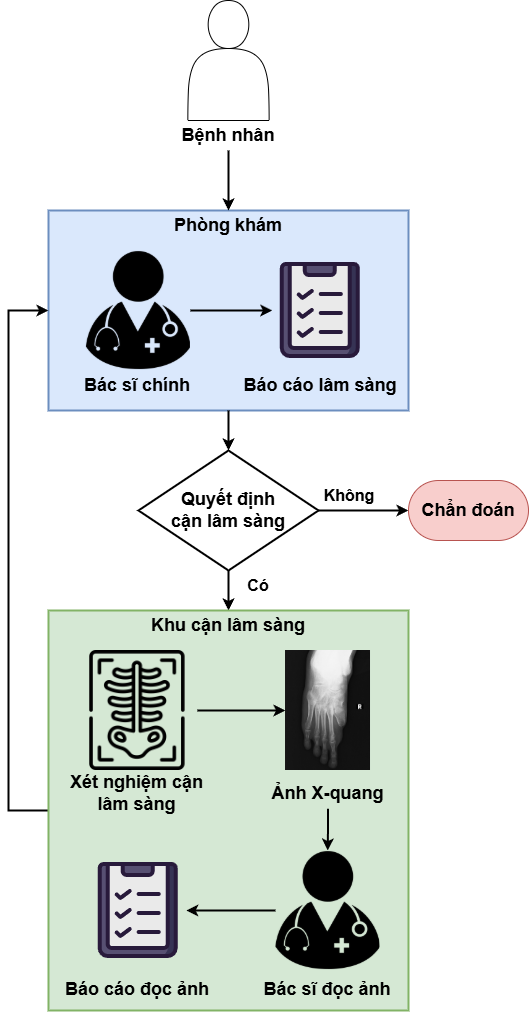
\includegraphics[width=0.8\linewidth]{images/diagram.png}
    \caption{Sơ đồ quy trình khám chữa bệnh giản hóa (Tham khảo từ quy trình thực tế tại Bệnh viện Nguyễn Tri Phương \cite{QuyTrinhBVNTP}).}
    \label{fig:diagram}
\end{figure}

\begin{figure}[H]
\centering
    \includegraphics[width=0.9\linewidth]{images/diagram_XBone_net.png}
    \caption{Sơ đồ tích hợp hệ thống hỗ trợ chẩn đoán.}
    \label{fig:diagram_XBone_net}
\end{figure}


\subsection{Ý nghĩa khoa học của đề tài}

Đề tài góp phần làm rõ hiệu quả của việc kết hợp dữ liệu ảnh X-quang và văn bản lâm sàng trong bài toán phân loại đa lớp. Thông qua việc khai thác đồng thời hai nguồn dữ liệu, nghiên cứu đánh giá khả năng cải thiện chất lượng biểu diễn và hiệu quả phân loại so với các phương pháp chỉ sử dụng một phương thức, qua đó cung cấp cơ sở cho việc phát triển các hệ thống hỗ trợ chẩn đoán tận dụng hiệu quả dữ liệu y tế đa phương thức.

Bên cạnh đó, nghiên cứu kế thừa và tinh chỉnh mô hình ngôn ngữ trực quan trên dữ liệu X-quang xương ở Việt Nam, góp phần đánh giá khả năng thích nghi của các mô hình tiền huấn luyện đa phương thức đối với các bài toán y khoa đặc thù ở Việt Nam và có quy mô dữ liệu hạn chế với phân bố mất cân bằng.

Ngoài ra, đề tài nghiên cứu các phương pháp nâng cao khả năng tổng quát hóa của mô hình trong điều kiện dữ liệu thực tế, đồng thời tích hợp cơ chế phát hiện dữ liệu ngoài phân phối. Cách tiếp cận này góp phần nâng cao độ tin cậy của hệ thống khi triển khai trong môi trường lâm sàng bằng cách hạn chế các dự đoán đối với những trường hợp chưa từng xuất hiện trong dữ liệu huấn luyện.

Cuối cùng, đề tài tăng cường khả năng giải thích của mô hình thông qua việc trực quan hóa các vùng ảnh X-quang có ảnh hưởng đến quá trình dự đoán, giúp bác sĩ chính hiểu rõ hơn cơ sở đưa ra kết quả phân loại và nâng cao tính minh bạch của hệ thống.

\subsection{Ý nghĩa thực tiễn của đề tài}

Hệ thống được đề xuất hướng đến hỗ trợ bác sĩ trong quá trình phân tích ảnh X-quang bằng cách kết hợp thông tin từ ảnh X-quang và dữ liệu lâm sàng ban đầu để đưa ra kết quả phân loại. Quá trình huấn luyện tận dụng báo cáo lâm sàng nhằm học mối quan hệ giữa ảnh X-quang và biểu hiện của bệnh lý. Cách tiếp cận này phù hợp với quy trình khám chữa bệnh thực tế tại các cơ sở y tế, góp phần nâng cao khả năng ứng dụng của hệ thống trong thực tiễn.

\pagebreak

Bên cạnh đó, hệ thống được thiết kế nhằm thích ứng với các đặc điểm phổ biến của dữ liệu y tế thực tế như số lượng mẫu gán nhãn hạn chế, phân bố dữ liệu mất cân bằng và sự xuất hiện của các trường hợp ngoài phân phối. 

Đồng thời, mô hình cung cấp các bản đồ nhiệt trực quan hóa vùng ảnh trong ảnh X-quang ảnh hưởng đến kết quả dự đoán và cơ chế cảnh báo đối với các mẫu dữ liệu ngoài phân phối, góp phần nâng cao tính minh bạch, độ tin cậy và tính an toàn khi hỗ trợ bác sĩ trong quá trình chẩn đoán.

\section{Giới thiệu bài toán}

Bài toán được nghiên cứu trong đề tài là bài toán phân loại đa lớp ảnh X-quang sử dụng học sâu đa phương thức. Mục tiêu của hệ thống là dự đoán các loại bệnh hoặc tổn thương dựa trên đồng thời dữ liệu hình ảnh X-quang và thông tin lâm sàng liên quan.

\begin{itemize}
  \item \textbf{Đầu vào:} Hệ thống nhận vào các nguồn dữ liệu sau:

  \begin{itemize}
    \item Ảnh X-quang của bệnh nhân:
\[ x^{img} \in \mathrm{R}^{H \times W \times C} \] trong đó:
    \begin{itemize}
        \item $H, W$: chiều cao và chiều rộng ảnh,
        \item $C$: số kênh màu của ảnh.
    \end{itemize}

    \item Thông tin lâm sàng (lời khai bệnh nhân, triệu chứng, tiền sử bệnh).
\[ x^{txt} = \{w_1, w_2, ..., w_T\} \] trong đó:
    \begin{itemize}
        \item $w_t$: từ thứ $t$,
        \item $T$: số lượng từ trong văn bản.
    \end{itemize}

    \item Tập nhãn được định nghĩa trước:
\[ \mathcal{Y} = \{y_1, y_2, ..., y_K\} \] với $K$ là số lớp bệnh cần phân loại.
  \end{itemize}

  \item \textbf{Đầu ra:} Hệ thống sinh ra:

  \begin{itemize}
    \item Cảnh báo dữ liệu ngoài phân phối/chưa từng gặp với các mẫu được hệ thống cho là không thuộc các lớp đã học.
    \item Nhãn dự đoán cuối cùng với các mẫu được cho là thuộc các lớp đã học:
    \[ \hat{y} = f(x^{img}, x^{txt}) \in \mathcal{Y} \] trong đó $f$ là hàm ánh xạ được học bởi mô hình.
    \item Bản đồ nhiệt trực quan hóa trên ảnh nhằm giải thích dự đoán của mô hình.
  \end{itemize}
\end{itemize}

\subsection{Các thách thức trong bài toán}

Mặc dù các mô hình học sâu đa phương thức đã đạt được nhiều kết quả tích cực, bài toán vẫn tồn tại nhiều thách thức cần được giải quyết:

\begin{itemize}
    \item Tồn tại sự chênh lệch lớn giữa các bộ dữ liệu đa phương thức hiện có (thường là cặp ảnh X-quang và báo cáo đọc ảnh X-quang)
so với luồng công việc thực tế lâm sàng (bao gồm ảnh chụp X-quang kết hợp với báo cáo tổng quát), làm hạn chế khả năng ứng dụng trực tiếp của các mô hình.
    \item Sự khác biệt về không gian và ngữ nghĩa giữa dữ liệu hình ảnh và dữ liệu văn bản gây khó khăn cho quá trình học biểu diễn chung, yêu cầu một cơ chế dung hợp hiệu quả.
    \item Dữ liệu y tế thường có số lượng hạn chế và mất cân bằng giữa các loại bệnh, đặt ra yêu cầu đặc biệt về thiết kế mô hình để tận dụng tối đa thông tin có sẵn.
    \item Trong thực tế lâm sàng, luôn có tỉ lệ xuất hiện những loại bệnh mới nằm ngoài dữ liệu huấn luyện, đặt ra yêu cầu về khả năng tổng quát hóa và thích ứng của mô hình.
    \item Khả năng giải thích của mô hình vẫn còn hạn chế khiến độ tin cậy vào các dự đoán của hệ thống là không cao, gây khó khăn cho việc triển khai trong thực tế lâm sàng.
\end{itemize}

\section{Mục tiêu nghiên cứu}
Đề tài hướng đến việc nghiên cứu và xây dựng một hệ thống học sâu đa phương thức phục vụ hỗ trợ phân loại bệnh lý trên ảnh X-quang xương, khai thác đồng thời dữ liệu hình ảnh và báo cáo lâm sàng nhằm đảm bảo hiệu quả phân loại so với các phương pháp hiện có và có khả năng thích ứng với các tình huống thực tế như dữ liệu ngoài phân phối và mất cân bằng lớp.

Các mục tiêu cụ thể của đề tài bao gồm:
\begin{enumerate}
  \item Đánh giá vai trò của báo cáo lâm sàng trong việc nâng cao hiệu quả phân loại bệnh lý xương khi kết hợp với ảnh X-quang, so với các phương pháp chỉ sử dụng dữ liệu hình ảnh.
  \item Nghiên cứu chiến lược dung hợp đặc trưng đa phương thức, cụ thể là cơ chế chú ý chéo và so sánh với các phương pháp khác, nhằm xác định phương pháp kết hợp hiệu quả giữa đặc trưng hình ảnh và văn bản.
  \item Khảo sát các phương pháp tinh chỉnh hiệu quả tham số, nhằm giảm chi phí tính toán trong khi duy trì hoặc cải thiện hiệu quả phân loại so với việc tinh chỉnh toàn bộ tham số.
  \item Nghiên cứu cơ chế phát hiện dữ liệu ngoài phân phối nhằm tăng khả năng nhận diện các mẫu bệnh lý chưa từng xuất hiện trong dữ liệu huấn luyện, nâng cao độ tin cậy của hệ thống trong môi trường thực tế.
  \item Xây dựng cơ chế giải thích dựa trên bản đồ chú ý giúp trực quan hóa các vùng ảnh mà mô hình tập trung khi đưa ra quyết định phân loại, hỗ trợ bác sĩ trong việc đánh giá và kiểm chứng kết quả dự đoán.
  \item Xây dựng và đánh giá hệ thống XBone-Net trên bộ dữ liệu phân loại bệnh lý xương có phân bố mất cân bằng, so sánh với các mô hình nền tảng y khoa hiện có.
\end{enumerate}

\section{Đối tượng và phạm vi nghiên cứu}
\subsection{Đối tượng nghiên cứu}
Đối tượng nghiên cứu của đề tài là các mô hình học sâu đa phương thức sử dụng đồng thời dữ liệu hình ảnh và văn bản trong bài toán phân loại ảnh X-quang xương. Cụ thể, nghiên cứu tập trung vào các thành phần chính sau:

\begin{itemize}
  \item Các mô hình ngôn ngữ trực quan tiền huấn luyện trên dữ liệu y khoa và dữ liệu tổng quát, được sử dụng làm bộ mã hóa đặc trưng đa phương thức.
  \item Các chiến lược dung hợp đặc trưng đa phương thức, bao gồm cơ chế chú ý chéo và phép nối đặc trưng, nhằm kết hợp thông tin từ ảnh X-quang và báo cáo lâm sàng.
  \item Các phương pháp tinh chỉnh tham số hiệu quả cho các mô hình tiền huấn luyện quy mô lớn nhằm giảm chi phí tính toán.
  \item Các kiến trúc bộ phân loại, phục vụ bài toán phân loại đa lớp trên dữ liệu mất cân bằng và phát hiện dữ liệu ngoài phân phối.
\end{itemize}

\subsection{Phạm vi nghiên cứu}
Đề tài tập trung vào bài toán phân loại đa lớp bệnh lý xương trên ảnh X-quang, kết hợp với báo cáo lâm sàng dạng văn bản. Phạm vi cụ thể bao gồm:

\begin{itemize}
  \item \textbf{Dữ liệu:} Nghiên cứu sử dụng bộ dữ liệu BTXRD gồm 10 lớp bệnh lý xương, và bộ dữ liệu CTCH được thu thập từ Bệnh viện Chấn thương Chỉnh hình Thành phố Hồ Chí Minh.
  \item \textbf{Dữ liệu văn bản:} Trong quá trình huấn luyện và suy luận, hệ thống sử dụng bệnh sử lâm sàng được thu nhận trước khi đọc ảnh (chứa thông tin triệu chứng và tiền sử bệnh) thay vì báo cáo đọc ảnh X-quang, nhằm hạn chế rò rỉ nhãn và phù hợp hơn với thời điểm áp dụng hệ thống.
  \item \textbf{Vai trò hệ thống:} Hệ thống được thiết kế làm công cụ hỗ trợ chẩn đoán, không thay thế vai trò của bác sĩ trong quá trình ra quyết định.
  \item \textbf{Giới hạn:} Đề tài không tập trung vào các bài toán phát hiện đối tượng, phân đoạn ảnh hay sinh báo cáo y khoa tự động.
\end{itemize}

\section{Các câu hỏi nghiên cứu và giả thuyết}
Trong các giả thuyết dưới đây, Macro F1-Score được sử dụng làm chỉ số chính cho bài toán phân loại do dữ liệu có phân bố mất cân bằng; Accuracy, Macro AUROC và Specificity được sử dụng làm các chỉ số bổ sung. Hiệu quả tính toán được đánh giá thông qua số tham số có thể huấn luyện, mức sử dụng bộ nhớ và thời gian suy luận. Đối với phát hiện dữ liệu ngoài phân phối, các chỉ số chính gồm AUROC, AUPR-Out và FPR@95TPR.

% Khi so sánh hai cấu hình trên cùng tập kiểm thử, mức cải thiện được xem là có ý nghĩa thống kê nếu khoảng tin cậy bootstrap 95\% của độ chênh lệch không chứa giá trị 0.

\begin{itemize}
    \item \textbf{Câu hỏi nghiên cứu 1:} Việc kết hợp bệnh sử lâm sàng được thu nhận trước khi đọc ảnh với ảnh X-quang có cải thiện hiệu quả phân loại so với mô hình chỉ sử dụng ảnh không?
    
    \textbf{Giả thuyết 1:} Mô hình sử dụng đồng thời ảnh X-quang và bệnh sử lâm sàng đạt Macro F1-Score cao hơn mô hình chỉ sử dụng ảnh trên cùng tập dữ liệu và quy trình đánh giá.

    \item \textbf{Câu hỏi nghiên cứu 2:} Cơ chế chú ý chéo hai chiều có khai thác tương tác giữa ảnh và văn bản hiệu quả hơn phép nối đặc trưng và các biến thể chú ý chéo một chiều không?

    \textbf{Giả thuyết 2:} Cơ chế chú ý chéo hai chiều đạt Macro F1-Score cao hơn các cấu hình dùng phép nối đặc trưng hoặc chỉ thực hiện chú ý theo một chiều khi các thành phần còn lại được giữ nguyên.

    \item \textbf{Câu hỏi nghiên cứu 3:} Chiến lược tinh chỉnh LoRA có duy trì hiệu quả phân loại trong khi giảm chi phí tính toán so với tinh chỉnh toàn bộ tham số không?
    
    \textbf{Giả thuyết 3:} LoRA đạt Macro F1-Score tương đương hoặc cao hơn tinh chỉnh toàn bộ tham số, đồng thời sử dụng ít tham số có thể huấn luyện và ít bộ nhớ hơn.

    \item \textbf{Câu hỏi nghiên cứu 4:} Nhánh xử lý ảnh độ phân giải cao dựa trên lưới ảnh cục bộ và bộ tái lấy mẫu có tọa độ có cải thiện khả năng phân loại so với các phương pháp chỉ sử dụng ảnh toàn cục hoặc co giãn ảnh không?

    \textbf{Giả thuyết 4:} Nhánh xử lý ảnh độ phân giải cao đạt Macro F1-Score cao hơn cấu hình chỉ sử dụng ảnh toàn cục và cấu hình co giãn ảnh khi sử dụng cùng backbone và chiến lược huấn luyện.

    \item \textbf{Câu hỏi nghiên cứu 5:} Hệ thống đề xuất XBone-Net có cải thiện hiệu quả phân loại so với các mô hình nền tảng được tinh chỉnh theo cùng cách thức đánh giá không?
     
    \textbf{Giả thuyết 5:} XBone-Net đạt Macro F1-Score cao hơn mô hình đối chứng tốt nhất; các chỉ số còn lại được báo cáo như tiêu chí bổ sung thay vì giả định XBone-Net phải vượt trội trên mọi độ đo.

    \item \textbf{Câu hỏi nghiên cứu 6:} Không gian biểu diễn của XBone-Net có hỗ trợ phân biệt dữ liệu nội phân phối với các bộ dữ liệu ngoài phân phối được xác định trước không?

    \pagebreak

    \textbf{Giả thuyết 6:} Ít nhất một phương pháp hậu xử lý được khảo sát, gồm khoảng cách Mahalanobis, Cosine-kNN, Energy Score và khoảng cách đến mốc văn bản, đạt AUROC lớn hơn mức ngẫu nhiên trong việc phân biệt dữ liệu nội phân phối và ngoài phân phối; phương pháp được lựa chọn dựa trên tập hiệu chỉnh thay vì tập kiểm thử.

    \item \textbf{Câu hỏi nghiên cứu 7:} Bản đồ chú ý của mô hình có tập trung vào các vùng tổn thương được chú thích trên ảnh X-quang không?

    \textbf{Giả thuyết 7:} Trên các mẫu có chú thích tổn thương, tỷ lệ khối lượng chú ý nằm trong vùng tổn thương lớn hơn tỷ lệ diện tích của vùng này trên ảnh, tương ứng với tỷ số tập trung chú ý lớn hơn 1.
\end{itemize}

\section{Đóng góp chính của đề tài}
Các đóng góp chính của đề tài bao gồm:

\begin{enumerate}
    \item \textbf{Quy trình sử dụng dữ liệu đa phương thức hạn chế rò rỉ nhãn:} Xây dựng quy trình sử dụng ảnh X-quang cùng bệnh sử lâm sàng được thu nhận trước khi đọc ảnh trong cả hai giai đoạn huấn luyện và khi suy luận. Báo cáo đọc ảnh, vốn có thể chứa trực tiếp kết luận chẩn đoán, được loại khỏi pipeline chính và chỉ được sử dụng trong các thí nghiệm loại bỏ thành phần nhằm đánh giá rò rỉ nhãn.

    \item \textbf{Kiến trúc XBone-Net xử lý ảnh độ phân giải cao:} Phát triển nhánh thị giác bao phủ toàn bộ ảnh X-quang bằng lưới ảnh cục bộ xác định, tổng hợp các token cục bộ và nén chúng bằng bộ tái lấy mẫu có sử dụng thông tin tọa độ. Biểu diễn thị giác sau đó được kết hợp với biểu diễn bệnh sử lâm sàng bằng cơ chế chú ý chéo hai chiều.

    \item \textbf{Quy trình huấn luyện hai giai đoạn với LoRA:} Thiết kế Giai đoạn 1 sử dụng Semantic Matching Loss để căn chỉnh biểu diễn ảnh và bệnh sử lâm sàng, sau đó tiếp tục tối ưu các adapter LoRA cùng mô-đun dung hợp trong Giai đoạn 2. Cách thiết kế này cho phép thích nghi mô hình BioMedCLIP với dữ liệu X-quang xương trong khi chỉ cập nhật một phần nhỏ tổng số tham số.

    \item \textbf{Bộ phân loại dựa trên tâm lớp thực nghiệm:} Xây dựng bộ phân loại phi tham số sử dụng độ tương đồng cosine đến các tâm lớp được ước lượng lại từ biểu diễn của tập huấn luyện. Trong Giai đoạn 2, mô hình được tối ưu bằng Cross-Entropy có trọng số theo số mẫu hiệu dụng nhằm giảm ảnh hưởng của phân bố lớp mất cân bằng.

    \item \textbf{Khung phát hiện dữ liệu ngoài phân phối:} Tích hợp quy trình phát hiện ngoài phân phối theo hướng hậu xử lý trên không gian biểu diễn đã học, hỗ trợ khoảng cách Mahalanobis, Cosine-kNN, Energy Score và khoảng cách đến mốc văn bản. Ngưỡng từ chối được hiệu chỉnh trên dữ liệu nội phân phối tách biệt trước khi đánh giá trên các bộ dữ liệu ngoài phân phối được xác định trước.

    \item \textbf{Công cụ phân tích khả năng giải thích:} Xây dựng công cụ trích xuất bản đồ chú ý đặc thù theo lớp từ mô-đun chú ý chéo hai chiều, chiếu trọng số chú ý ngược về các vùng ảnh gốc thông qua bộ tái lấy mẫu không gian và định lượng mức độ tập trung trên vùng tổn thương được chú thích. Công cụ này hỗ trợ phân tích hành vi của mô hình, không được xem là bằng chứng thay thế cho đánh giá lâm sàng của bác sĩ.
\end{enumerate}

\section{Bố cục luận văn}

\textbf{Chương 1: Giới thiệu.} Chương này cung cấp cái nhìn tổng quan về bối cảnh nghiên cứu, xác định rõ vấn đề cần giải quyết, mục tiêu, phương pháp tiếp cận và những đóng góp chính của đề tài. Đây là phần nền tảng định hướng cho toàn bộ nội dung khóa luận.

\textbf{Chương 2: Các công trình nghiên cứu liên quan.} Chương này tập trung hệ thống hóa các hướng tiếp cận đã được mô tả ở trên, làm tiền đề cho việc xây dựng giải pháp của khóa luận. Trọng tâm của chương là việc phân tích các kiến trúc mô hình ngôn ngữ trực quan cùng các chiến lược dung hợp đặc trưng đa phương thức. Bên cạnh đó, các kỹ thuật tinh chỉnh tối ưu và phương pháp nhận diện dữ liệu ngoài phân phối cũng được xem xét toàn diện, từ đó thiết lập cơ sở lý thuyết vững chắc và định vị rõ ràng hướng giải quyết của đề tài so với các công trình đi trước.

\textbf{Chương 3: Phương pháp đề xuất.} Đây là chương trọng tâm mô tả chi tiết quy trình xây dựng hệ thống. Tại đây, nhóm sẽ trình bày cụ thể về kiến trúc mô hình được kế thừa, quy trình xử lý dữ liệu đầu vào (cả ảnh và văn bản), thiết kế các hàm mất mát, và chiến lược huấn luyện mô hình. Các sơ đồ khối và thuật toán sẽ được mô tả chi tiết để minh họa cho giải pháp.

\textbf{Chương 4: Thực nghiệm và Kết quả.} Chương này trình bày về bộ dữ liệu được sử dụng, thiết lập môi trường thực nghiệm và các chỉ số đánh giá. Kết quả thực nghiệm sẽ được phân tích, so sánh đối chiếu với các phương pháp khác để làm rõ ưu nhược điểm của mô hình đề xuất.

\textbf{Chương 5: Kết luận và Hướng phát triển.} Chương cuối cùng tổng kết lại những kết quả đạt được so với mục tiêu ban đầu, nhìn nhận những hạn chế còn tồn tại của hệ thống và đề xuất các hướng nghiên cứu tiếp theo để hoàn thiện và mở rộng ứng dụng trong tương lai.
